\documentclass[tikz,border=3pt]{standalone}
\usepackage[utf8]{inputenc}
\usepackage[T1]{fontenc}
\usepackage{lmodern}
\renewcommand{\familydefault}{\sfdefault}
\usepackage{sansmath}\sansmath
\usepackage{chemfig}
\usepackage{pgfplots}\pgfplotsset{compat=1.18,/pgf/number format/use comma,/pgf/number format/1000 sep={.}}
\usetikzlibrary{arrows.meta,calc,positioning,decorations.pathmorphing,patterns}
% paleta del sitio
\definecolor{nar}{HTML}{E8680C}\definecolor{narc}{HTML}{FFB35C}\definecolor{hielo}{HTML}{FFF3E8}
\definecolor{tinta}{HTML}{1D1D1F}\definecolor{gris}{HTML}{6E6E73}\definecolor{lila}{HTML}{7C5CF0}
\definecolor{azul}{HTML}{2F6FD6}\definecolor{menta}{HTML}{17A673}\definecolor{coral}{HTML}{E8342A}
\begin{document}
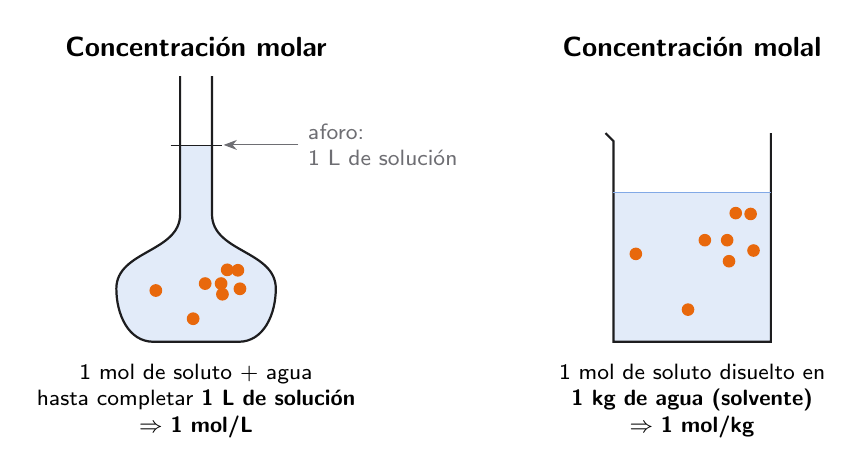
\begin{tikzpicture}[font=\small]
% --- molar: matraz aforado de 1 L
\begin{scope}[scale=1.35]
\path[fill=azul!14] (-0.15,1.85) -- (-0.15,1.2) to[out=-90,in=90] (-0.75,0.5) to[out=-90,in=180] (-0.4,0) -- (0.4,0)
   to[out=0,in=-90] (0.75,0.5) to[out=90,in=-90] (0.15,1.2) -- (0.15,1.85) -- cycle;
\draw[tinta,thick] (-0.15,2.5) -- (-0.15,1.2) to[out=-90,in=90] (-0.75,0.5) to[out=-90,in=180] (-0.4,0) -- (0.4,0)
   to[out=0,in=-90] (0.75,0.5) to[out=90,in=-90] (0.15,1.2) -- (0.15,2.5);
\draw[tinta] (-0.24,1.85) -- (0.24,1.85);
\pgfmathsetseed{3}
\foreach \i in {1,...,8} {\fill[nar] ($(0,0)+(-0.45+0.9*rnd,0.12+0.6*rnd)$) circle (0.06);}
\end{scope}
\draw[gris,-{Stealth}] (1.3,2.5) -- (0.35,2.5) node[pos=0,right,font=\footnotesize,align=left] {aforo:\\1 L de solución};
\node[font=\bfseries] at (0,3.75) {Concentración molar};
\node[align=center,font=\footnotesize] at (0,-0.75) {1 mol de soluto + agua\\hasta completar \textbf{1 L de solución}\\$\Rightarrow$ \textbf{1 mol/L}};
% --- molal: vaso con 1 kg de agua
\begin{scope}[shift={(6.3,0)}]
\fill[azul!14] (-1,0) rectangle (1,1.9);
\draw[tinta,thick] (-1.1,2.65) -- (-1,2.55) -- (-1,0) -- (1,0) -- (1,2.65);
\draw[azul!60] (-1,1.9) -- (1,1.9);
\pgfmathsetseed{3}
\foreach \i in {1,...,8} {\fill[nar] ($(0,0)+(-0.85+1.7*rnd,0.15+1.6*rnd)$) circle (0.08);}
\end{scope}
\node[font=\bfseries] at (6.3,3.75) {Concentración molal};
\node[align=center,font=\footnotesize] at (6.3,-0.75) {1 mol de soluto disuelto en\\\textbf{1 kg de agua (solvente)}\\$\Rightarrow$ \textbf{1 mol/kg}};
\end{tikzpicture}
\end{document}
